\documentclass{article}
\usepackage[utf8]{inputenc}
\usepackage{enumitem}
\usepackage{graphicx}

\title{440 Assignment 3}
\author{Xiaowei Zhang, 204007085 \\ Xinyuan Chen, 197001668}
\date{December 2021}

\begin{document}
\maketitle

\section*{Problem 1}
Game tree see Figure 1. We don't care about the "?" values because when we use the MINIMAX strategy, at state $(3,2)$, it's B's turn, so we apply MIN, then the path to state $(2,4)$ will be pruned. Also, at state $(2,3)$, it's A's turn, so we apply MAX, then the path to state $(1,4)$ will be pruned.
\begin{figure}
        \centering
        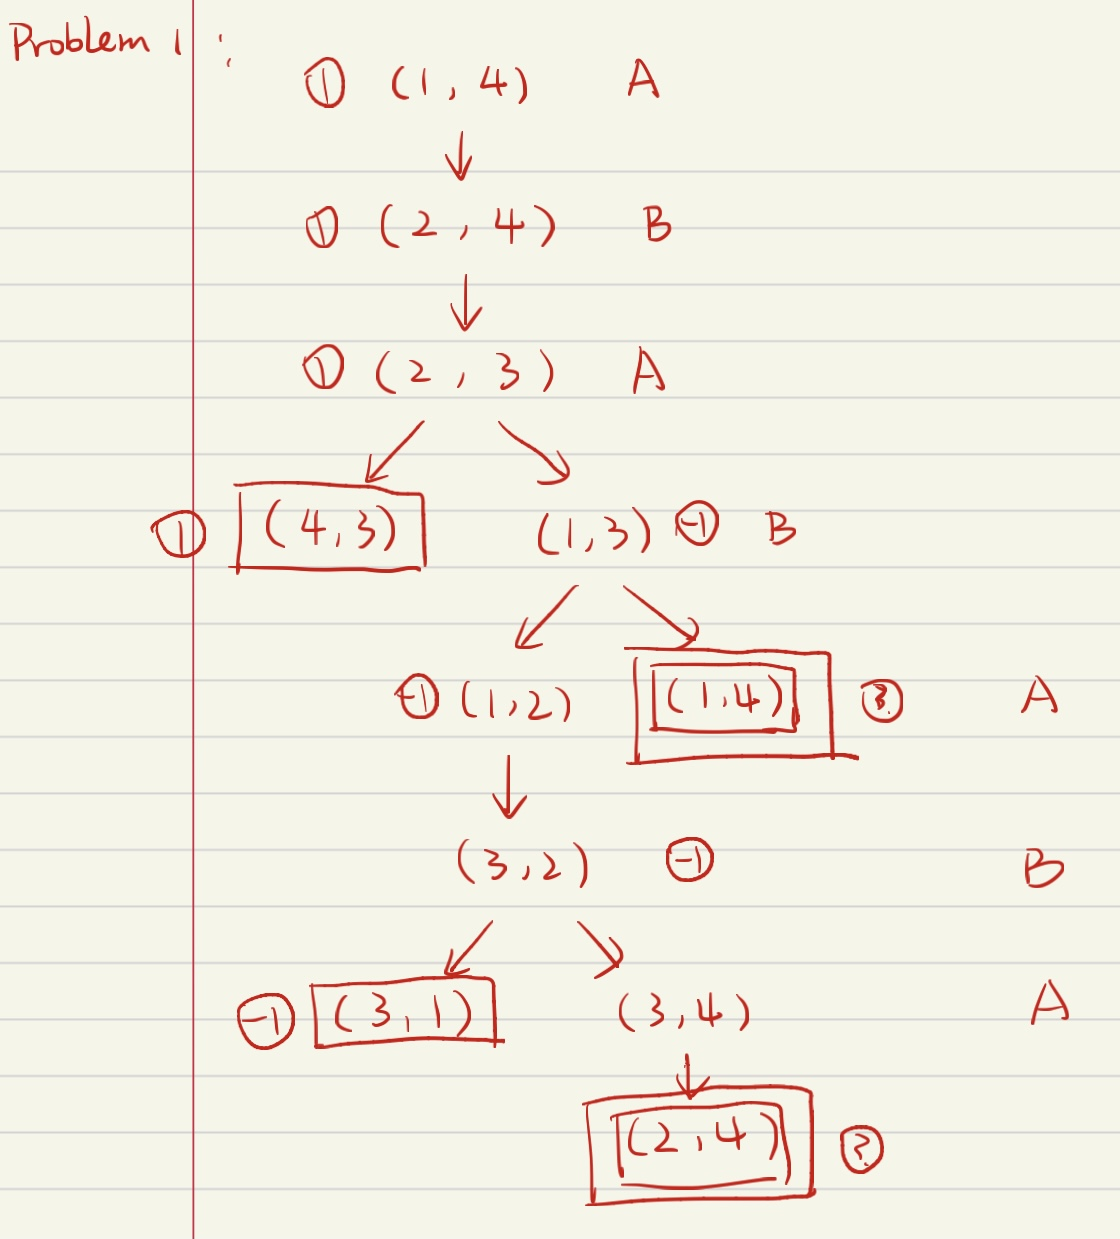
\includegraphics[width=0.8\textwidth]{problem1.jpg}
        \caption{Game Tree}
\end{figure}

\section*{Problem 2}
\begin{enumerate}[label=\alph*)]
\item
    $P(A, B, C, D, E) \\
    &= P(A) \cdot P(B)\cdot P(C)\cdot P(D|A,B)\cdot P(E|B,C) \\
    &= 0.2 * 0.5 * 0.8 * 0.1 * 0.3 \\
    &= 0.0024$
\item
   $P(\neg A, \neg B, \neg C, \neg D, \neg E) \\
   &= P(\neg A)\cdot P(\neg B)\cdot P(\neg C)\cdot P(\neg D|\neg A, \neg B)\cdot P(\neg E|\neg B, \neg C) \\
   &= 0.8 * 0.5 * 0.2 * 0.1 * 0.8 \\
   &= 0.0064$ 
\item $P(\neg A|B, C, D, E)\\
   &= \alpha \cdot P(\neg A, B, C, D, E) \\
   &= \alpha \cdot (0.8*0.5*0.8*0.6*0.3) \\
   &= \alpha \cdot 0.0576$\\
   $\alpha 
   &= \frac{1}{P(A, B, C, D, E)+P(\neg A, B, C, D, E)} \\
   &= \frac{1}{(0.2*0.5*0.8*0.1*0.3)+(0.8*0.5*0.8*0.6*0.3)}\\
   &= \frac{1}{0.0024+0.0576}\\
   &= \frac{50}{3}$\\
Thus $P(\neg A|B, C, D, E) \\
   &= \frac{50}{3} * 0.0576 \\
   &= 0.96$


\end{enumerate}

\section*{Problem 3}
\begin{enumerate}[label=\alph*)]
\item
$P(B|j,m) \\
&= \alpha P(B,j,m) \\
&= \alpha \sum_e \sum_a P(B,j,m,e,a) \\$
For $B = true$:\\
$P(b|j,m) \\
&= \alpha \sum_e \sum_a P(b)P(e)P(a|b,e)P(j|a)P(m|a) \\
&= \alpha P(b) \sum_e P(e) \sum_a P(a|b,e)P(j|a)P(m|a)\\
&= \alpha [P(b)P(e)P(a|b,e)P(j|a)P(m|a) \,+\, P(b)P(\neg e)P(a|b,\neg e)P(j|a)P(m|a) \,+\, P(b)P(e)P(\neg a|b,e)P(j|\neg a)P(m|\neg a) \,+\, P(b)P(\neg e)P(\neg a|b,\neg e)P(j|\neg a)P(m|\neg a)]\\
&= \alpha[(0.001*0.002*0.95*0.9*0.7) + (0.001*0.998*0.94*0.9*0.7) + (0.001*0.002*0.05*0.05*0.01) + (0.001*0.998*0.06*0.05*0.01)]\\
&= \alpha \cdot 0.00059224$\\
For $B = false$:\\
$P(\neg b|j,m) \\
&= \alpha \sum_e \sum_a P(\neg b)P(e)P(a|\neg b,e)P(j|a)P(m|a) \\
&= \alpha P(\neg b) \sum_e P(e) \sum_a P(a|\neg b,e)P(j|a)P(m|a)\\
&= \alpha [P(\neg b)P(e)P(a|\neg b,e)P(j|a)P(m|a) \,+\, P(\neg b)P(\neg e)P(a|\neg b,\neg e)P(j|a)P(m|a) \,+\, P(\neg b)P(e)P(\neg a|\neg b,e)P(j|\neg a)P(m|\neg a) \,+\, P(\neg b)P(\neg e)P(\neg a|\neg b,\neg e)P(j|\neg a)P(m|\neg a)]\\
&= \alpha[(0.999*0.002*0.29*0.9*0.7) + (0.999*0.998*0.001*0.9*0.7) + (0.999*0.002*0.71*0.05*0.01) + (0.999*0.998*0.999*0.05*0.01)]\\
&= \alpha \cdot 0.00149194$\\
$\alpha = \frac{1}{P(b,j,m)+P(\neg b,j,m)}$\\
Thus $P(B|j,m) = \alpha <0.00059224,0.00149194> \,\approx\, <0.284,0.716>$

% &= \alpha \cdot \left[ \begin{array}{c} 0.001 \\ 0.999 \end{array} \right]
\item
The complexity of computing $P(X_1|X_n=true)$ using enumeration is $O(2^n)$, and the complexity using variable elimination is $O(n)$.
\end{enumerate}

\section*{Problem 4}
    OC : card holder owns a computer or smart phone.\\
	Fraud : current transaction is fraudulent.\\
	Trav : card holder is currently travelling.\\
	FP : current transaction is a foreign purchase.\\
	IP : current purchase is an internet purchase.\\
	CRP : a computer related purchase was made in the past week.\\
	$P(Frau|Trav) = 0.01$, $P(Frau|\neg Trav) = 0.004$\\
	$P(Trav) = 0.05$\\
	$P(FP|\neg Trav,Fraud) = 0.1$, $P(FP|\neg Trav,\neg Fraud) = 0.01$\\
	$P(FP|Trav) = 0.9$\\
	$P(OC)=0.75$\\
	$P(IP|OC,\neg Fraud) = 0.01$, $P(IP|OC, Fraud) = 0.02$\\
	$P(IP|\neg OC,\neg Fraud) = 0.001$, $P(IP|\neg OC,Fraud) = 0.011$\\
	$P(CRP|OC) = 0.1$, $P(CRP|\neg OC) = 0.001$
\begin{enumerate}[label=\alph*)]
\item Bayes Network see Figure 2.
\begin{figure}
        \centering
        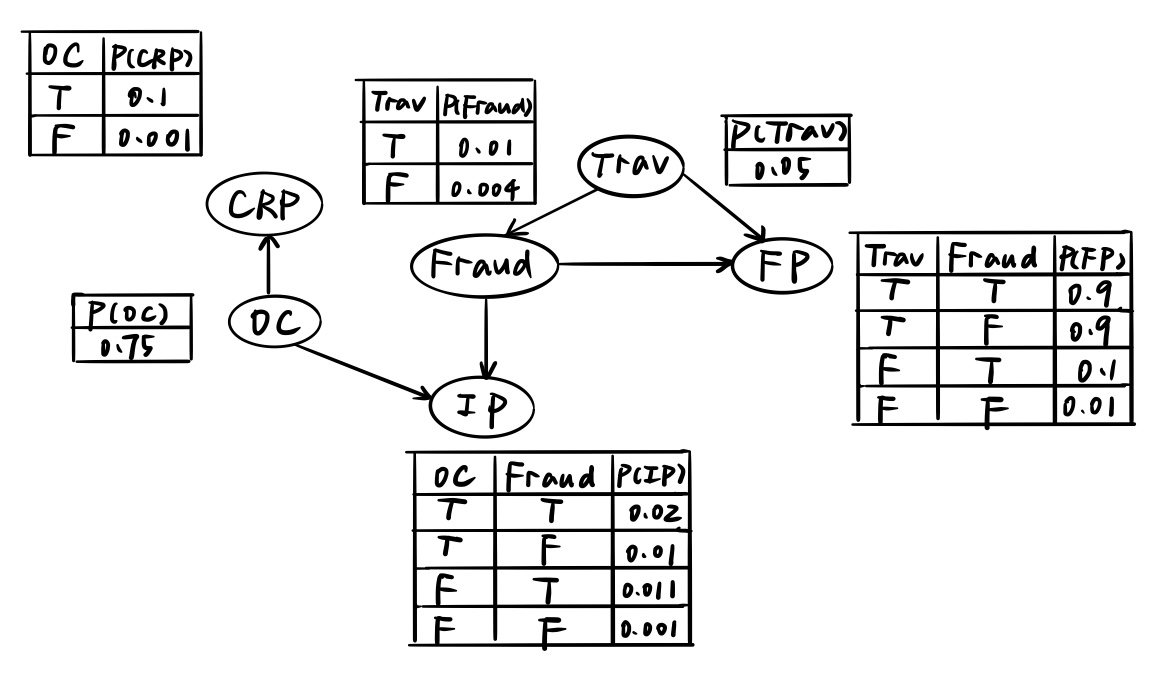
\includegraphics[width=1\textwidth]{problem4.jpg}
        \caption{Bayes Network}
\end{figure}
\item
$P(Fraud)\\
&= P(Fraud|Trav)P(Trav) + P(Fraud|\neg Trav)P(\neg Trav)\\
&= (0.01*0.05) + (0.004*0.95)\\
&= 0.0043$\\
$P(Fraud|FP, \neg IP, CRP)\\
&= \frac{P(Fraud, FP, \neg IP, CRP)}{P(FP, \neg IP, CRP)}
$\\
$P(Fraud, FP, \neg IP, CRP)\\
&= \sum_{OC} \sum_{Trav} P(Trav)P(FP|Trav,Fraud)P(\neg IP| OC,Fraud)P(CRP|OC)P(Fraud|Trav)\\
&= 0.05*0.9*0.98*0.1*0.01 + 0.95*0.1*0.98*0.1*0.004 + 0.05*0.9*0.989*0.001*0.01 + 0.95*0.1*0.989*0.001*0.004\\
&= 0.00008216087$\\
$P(\neg Fraud, FP, \neg IP, CRP)\\
&= \sum_{OC} \sum_{Trav} P(Trav)P(FP|Trav,\neg Fraud)P(\neg IP| OC,\neg Fraud)P(CRP|OC)P(\neg Fraud|Trav)\\
&= 0.05*0.9*0.99*0.1*0.99 + 0.95*0.01*0.99*0.1*0.996 + 0.05*0.9*0.999*0.001*0.99 + 0.95*0.01*0.999*0.001*0.996\\
&= 0.005445651438$\\
$P(Fraud|FP, \neg IP, CRP)\\
&= \frac{0.00008216087}{0.00008216087+0.005445651438}\\
&= 0.01486318012
$
\end{enumerate}
\end{document}